\begin{frame}
  %\frametitle{}
  \begin{columns}[t]
    \column{.5\textwidth}
    \begin{block}{}%A general class of PDE}
      \begin{itemize}
      \item{
	Associated to the problem domain $\Omega$ is a LibMesh data
	structure called a \texttt{Mesh}
      }
	
      \item{A \texttt{Mesh} is essentially
	a collection of finite elements}
      \end{itemize}
      \begin{equation}
	\label{eqn:discretized_domain}
	\nonumber
	\Omega^h:=\bigcup_e \Omega_e
      \end{equation}
    \end{block}
    %\pause
    \column{.5\textwidth}
    %\begin{block}{}
      \begin{center}
	%\fbox{
	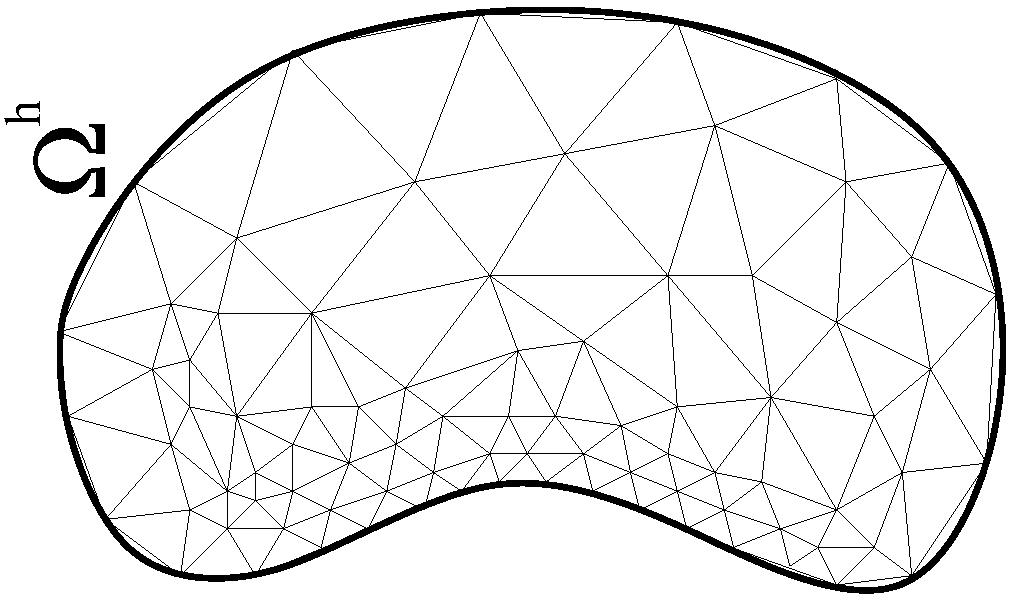
\includegraphics[width=2in,angle=-90]{discretized_domain}
	%}
      \end{center}
    %\end{block}
  \end{columns}
  \visible<2>
  {
  \begin{itemize}
    \item{LibMesh provides some simple structured mesh generation
routines, file inputs, and interfaces to Triangle and TetGen.}
  \end{itemize}
  }
\end{frame}


%% \begin{frame}
%%   \frametitle{The Mesh}
%%   \begin{block}{}
%%     The \texttt{Mesh} data structure provides: 
%%     \begin{itemize}
%%     \item{Iterator access to the nodes and elements}
%%     \end{itemize}
%%   \end{block}
%% \end{frame}
